\documentclass{article}
\usepackage{graphicx}

\begin{document}

\title{COP290 Rust Lab: Spreadsheet + Extension}
\author{\textbf{Laksh Goel (2023CS10848)} 
\\ \textbf{Adit Jindal (2023CS50626)} \\ \textbf{Yuvika Chaudhary (2023CS10353)}}
\maketitle
\section{About the Project}

We have developed a versatile and feature-rich spreadsheet application in Rust that supports a command-line (terminal) interface and a web-based interface (mainly for display). This dual-interface design allows users to interact with spreadsheets in the environment that best suits their preferences, either directly in the terminal or through a graphical web interface in the browser.
\subsection*{Terminal Interface}

The terminal interface provides a keyboard-driven experience for managing a grid of integer-valued cells. Users can:
\begin{itemize}
\item Assign values to cells directly or via the following types of formulas:
\begin{enumerate}
\item Constants or references to other cells
\item Arithmetic expressions (addition, subtraction, multiplication, division)
\item Range-based functions such as \texttt{SUM}, \texttt{AVG}, \texttt{MIN}, \texttt{MAX}, and \texttt{STDEV}
\end{enumerate}
\item Reference both one-dimensional and two-dimensional cell ranges in formulas
\item Navigate large spreadsheets efficiently using commands (\texttt{w}, \texttt{a}, \texttt{s}, \texttt{d}) and jump to specific cells
\item See execution time for each command and receive clear error messages for invalid inputs.
\end{itemize}
The terminal version emphasizes responsive parsing, real-time dependency updates, and robust cycle detection to prevent circular references.

\subsection*{Terminal and Web Extension}

Inside the Terminal, feature additions are:
\begin{enumerate}
    \item Track and reverse changes using undo/redo functionality
    \item Save to and load spreadsheets from JSON format for saving custom nodes, which allows preservation of dependencies among cells.
    \item A web based display module for data analysis. It allows unit-changes only.
\end{enumerate}

The web extension brings a modern, graphical spreadsheet experience to the browser, leveraging Rust compiled to WebAssembly (WASM) for performance and safety. Its key features include:
\begin{itemize}
\item Intuitive cell editing and formula entry through a graphical user interface
\item Mouse-based range selection and navigation
\item Dynamic charting and data visualization, including pixel art/image generation from spreadsheet data (heat maps)
\item Undo/redo functionalities
\item Theme switching (light/dark mode)
\item JSON import/export for seamless data transfer between terminal and web versions
\item Real-time updates and error feedback
\item Shared backend logic with the terminal version for consistency
\end{itemize}
The extension is structured with a clear separation between backend logic (grid management, dependency tracking, formula evaluation) and frontend components (UI rendering, user interaction), communicating efficiently via browser APIs and WASM bindings.

\section{Built With}
The main data structures and concepts used in the Rust implementation are
\begin{enumerate}
    \item \textbf{Dependency Graph}: The spreadsheet is modeled as a dependency graph, where each cell is a \texttt{Node}. E.g., if Cell1 depends on Cell2, a directed edge is formed from Cell2 to Cell1. This structure enables automatic propagation of updates and robust cycle detection. This dependency is stored in the Node, which gets stored in the JSON files used for serialization.
    \item \textbf{Vectors (\texttt{Vec})}: Rust's dynamic arrays are used for storing the grid of cells, lists of dependents, and for efficiently managing collections whose size may change at runtime.
    \item \textbf{Strong Typing and Enums}: Custom structs and enums (such as \texttt{Node}, \texttt{Coordinates}, and \texttt{Operation}) provide clarity and safety in representing cells, positions, and supported operations.
    \item \textbf{Efficient Evaluation}: The backend uses topological sorting to update dependent cells in the correct order whenever a value changes, ensuring consistency and performance.
    \item \textbf{Error Handling}: Rust's type system and explicit validity flags in each node ensure that errors (such as invalid references, cycles, or division by zero) are detected and reported without crashing the program unless necessary.
    \item \textbf{Extensible Parsing}: A modular parser interprets user commands, supporting a wide range of expressions and functions, and can be easily extended for new features.
\end{enumerate}

\noindent
\textbf{Additional Features:}
\begin{itemize}
    \item Dual interface: Both terminal and web-based interfaces (with the web extension supporting advanced features like charts and pixel art)
    \item Undo/Redo: Track and revert changes to the spreadsheet
    \item JSON Import/Export: Save and load spreadsheet states
    \item Data Visualization: Generate images and charts from spreadsheet data (web interface)
\end{itemize}

\noindent
The Rust implementation leverages safe and efficient data structures from the standard library, ensuring both performance and maintainability.

\section{Project Structure}

The project is organized into well-defined modules to support both terminal and web-based spreadsheet interfaces, while also handling efficient command parsing and the backend logic. Below is a description of the main directories and files, based on the current repository structure:

\begin{itemize}
    \item \texttt{terminal/}: Implements the terminal-based spreadsheet interface and its backend logic.
    \begin{itemize}
        \item \texttt{backend.rs}: Core spreadsheet logic, including grid management, dependency updates, evaluation, and cycle detection.
        \item \texttt{graph.rs}: Data structures and methods for the dependency graph and cell nodes.
        \item \texttt{functions.rs}: Definitions for arithmetic and range functions (SUM, AVG, MIN, MAX, STDEV, etc.) and operation enums.
        \item \texttt{parser.rs}: Parses and validates user commands.
        \item \texttt{spreadsheet.rs}: Handles user interaction, grid rendering, and command execution in the terminal.
        \item \texttt{types.rs}: Common types such as \texttt{Coordinates} for cell positions.
        \item \texttt{mod.rs}: Module declarations for the terminal package.
    \end{itemize}
    \item \texttt{extension/}: Contains the terminal integrated with the web-based spreadsheet implementation.
    \begin{itemize}
        \item \texttt{backend/}: Backend logic for the web extension, mirroring the terminal backend structure.
        \begin{itemize}
            \item \texttt{backend.rs}, \texttt{functions.rs}, \texttt{graph.rs}, \texttt{mod.rs}: Same responsibilities as their terminal counterparts, adapted for the web, for the sake of consistency.
        \end{itemize}
        \item \texttt{frontend/}: Frontend components for the web user interface.
        \begin{itemize}
            \item \texttt{terminal.rs}: Terminal-like interface to manipulate and create spreadsheets to be displayed on the web as required.
            \item \texttt{web.rs}: Main web UI logic.
            \item \texttt{mod.rs}: Module declarations for the frontend.
        \end{itemize}
        \item \texttt{parser/}: Command parsing logic shared by the web extension.
        \begin{itemize}
            \item \texttt{parser.rs}: Command parsing and validation.
            \item \texttt{common.rs}: Shared parsing utilities.
            \item \texttt{mod.rs}: Module declarations for the parser.
        \end{itemize}
        \item \texttt{mod.rs}: Module declarations for the extension package.
    \end{itemize}
    \item \texttt{lib.rs}: Library root for shared logic.
    \item \texttt{main.rs}: Entry point for the purely-terminal based application (from C Lab).
    \item \texttt{extension\_main.rs}: Entry point for the extension.
\end{itemize}

\noindent
The modular structure ensures code reusability and maintainability, allowing both terminal and web interfaces to share core logic while providing interface-specific features.


\section{Terminal Architecture}
The spreadsheet application is structured around two main data abstractions: the \textbf{graph} (dependency graph of cells) and the \textbf{grid} (the table of cell values and operations). The following components define the architecture:

\begin{enumerate}
\item \textbf{graph}: A two-dimensional vector (\texttt{Vec<Vec<Node>>}) representing the spreadsheet's dependency graph. Each element is a \texttt{Node} struct corresponding to a cell, and the graph encodes dependencies between cells for correct evaluation order and cycle detection.
\item \textbf{grid}: The same 2D vector of \texttt{Node}s serves as both the dependency graph and the value grid, with each node storing its computed value, operation, and dependency metadata.
\item \textbf{Node}: A custom struct (\texttt{Node}) encapsulating:
\begin{itemize}
\item \texttt{node\_value}: The computed integer value of the cell.
\item \texttt{value1}, \texttt{value2}: Operands for the cell's operation, represented as \texttt{Coordinates} (for cell references) or as constants (with column set to \texttt{-1}).
\item \texttt{op}: The operation performed by the cell, as an \texttt{Operation} enum (e.g., Add, Sub, Sum, etc.).
\item \texttt{dependents}: A vector of \texttt{Coordinates} for all cells that depend on this cell.
\item \texttt{valid}: Boolean flag indicating if the cell's value is currently valid.
\item \texttt{visited}: Boolean flag used for traversal algorithms (e.g., cycle detection, topological sort).
\item \texttt{position}: The cell's own coordinates in the grid.
\end{itemize}
\item \textbf{value1, value2}: Instances of \texttt{Coordinates} within each \texttt{Node}, representing either:
\begin{itemize}
\item The start and end cells of a range (for range operations).
\item The two operand cells (for binary operations).
\item A constant value (with column set to \texttt{-1}).
\end{itemize}
\item \textbf{Coordinates}: A struct (\texttt{Coordinates}) containing two \texttt{i32} fields: \texttt{row} and \texttt{col}, representing the position of a cell in the grid.
\item \textbf{Operation}: An enum (\texttt{Operation}) listing all supported cell operations, including arithmetic (Add, Sub, etc.), range functions (Sum, Avg, etc.), and special commands (Sleep, EnableOutput, etc.).
\item \textbf{Dependency Management}: Each \texttt{Node} maintains a list of its outward dependencies (cells that depend on it) via the \texttt{dependents} vector. Dependency edges are updated as formulas change, and cycles are detected using depth-first traversal with the \texttt{visited} flag.
\item \textbf{Evaluation and Topological Sorting}: When a cell is updated, the dependency graph is traversed in topological order to recompute all affected cells. The \texttt{evaluate\_node} function handles computation, supporting both cell references and constants.
\item \textbf{Parser and Frontend}: User commands are parsed into operations and operands, which are then dispatched to the backend for processing. The frontend handles grid display and user interaction.
\end{enumerate}

\textbf{Note:} Unlike the C implementation, which used a custom hash table for outward dependencies, the Rust version uses a vector of \texttt{Coordinates} for each node's dependents, leveraging Rust's safe and efficient collections.


\section{Extension Architecture}
We have extended the project described above to add more functions to it and make it more relevant to a real-world user. This involves having features for saving and opening a saved file in a custom format, undoing and redoing commands, and displaying the sheet in a web-based GUI for better data analytics.
The features added are thus:
\begin{enumerate}
    \item \textbf{Undo-Redo stack}: All executed operations are stored in a stack. This allows the user to run $undo$ to revert the last change, and running $redo$ brings the change back, along with its dependencies. This allows reverting errors, making the program more useful. 
    The stack has an upper limit of 1000, so up to one thousand commands can be undone.
    \item \textbf{Serialization}: We can save the sheet formed in a JSON file. For this, the user needs to run $save myfile.json$, by replacing 'myfile' with the desired name. This file gets saved in the project directory directly, and the sheet can be further worked upon. This feature can be used as a simpler substitute for version control, though not completely replacing it. The JSON file formed contains descriptions of all nodes in the table, thus preserving dependencies.
    \item \textbf{Deserialization}: Once a file has been saved using the above-described command, it can be opened again later and continued to be worked upon. For this, while running the executable, additional arguments need to be passed in the terminal. The first two arguments are taken to be the dimensions (rows and columns), and the third optional argument is the file to be opened.\\ e.g., for a file named 'myfile.json', the following command will work: \texttt{./"executable" 5 6 myfile.json}.\\ This will open the file in the terminal interface, along with all the dependencies preserved.\\The dimensional arguments in the command serve as safety, in case the file is not accessible or does not form a sheet properly. In such a case, the dimensions passed are used to create a new sheet, completely ignoring the file.
    \item \textbf{Web-based display}: We also have a web-based GUI, intended for data analysis. It allows several features and operations, as specified below. The GUI can be accessed by two means:
    \begin{enumerate}
        \item \texttt{web\_start}: This opens the current state of the sheet in the web.
        \item \texttt{web myfile.json}: This opens a pre-existing file in the web, rather than the current state in the terminal.
    \end{enumerate}
    The GUI is intended only for analyzing the current state, and to try out unit changes in it and observe their effects. For this reason, it allows only one change at a time, that is, making a second change undoes the first. It allows the user to undo the last command performed in the sheet (again, up to a depth of one).
\end{enumerate}

\section{Features of the web-display}
\begin{enumerate}
    \item Displays the table in a more interactive manner. Lets the user select the range of rows and columns to display, thus allowing focus on the required sections of data alone.
    \item Allows selection of ranges of cells(1D or 2D), which displays statistics for the selected range. The statistics include the mean, sum, maximum, minimum and standard deviation.
    \begin{figure}[t]
    \centering
    {{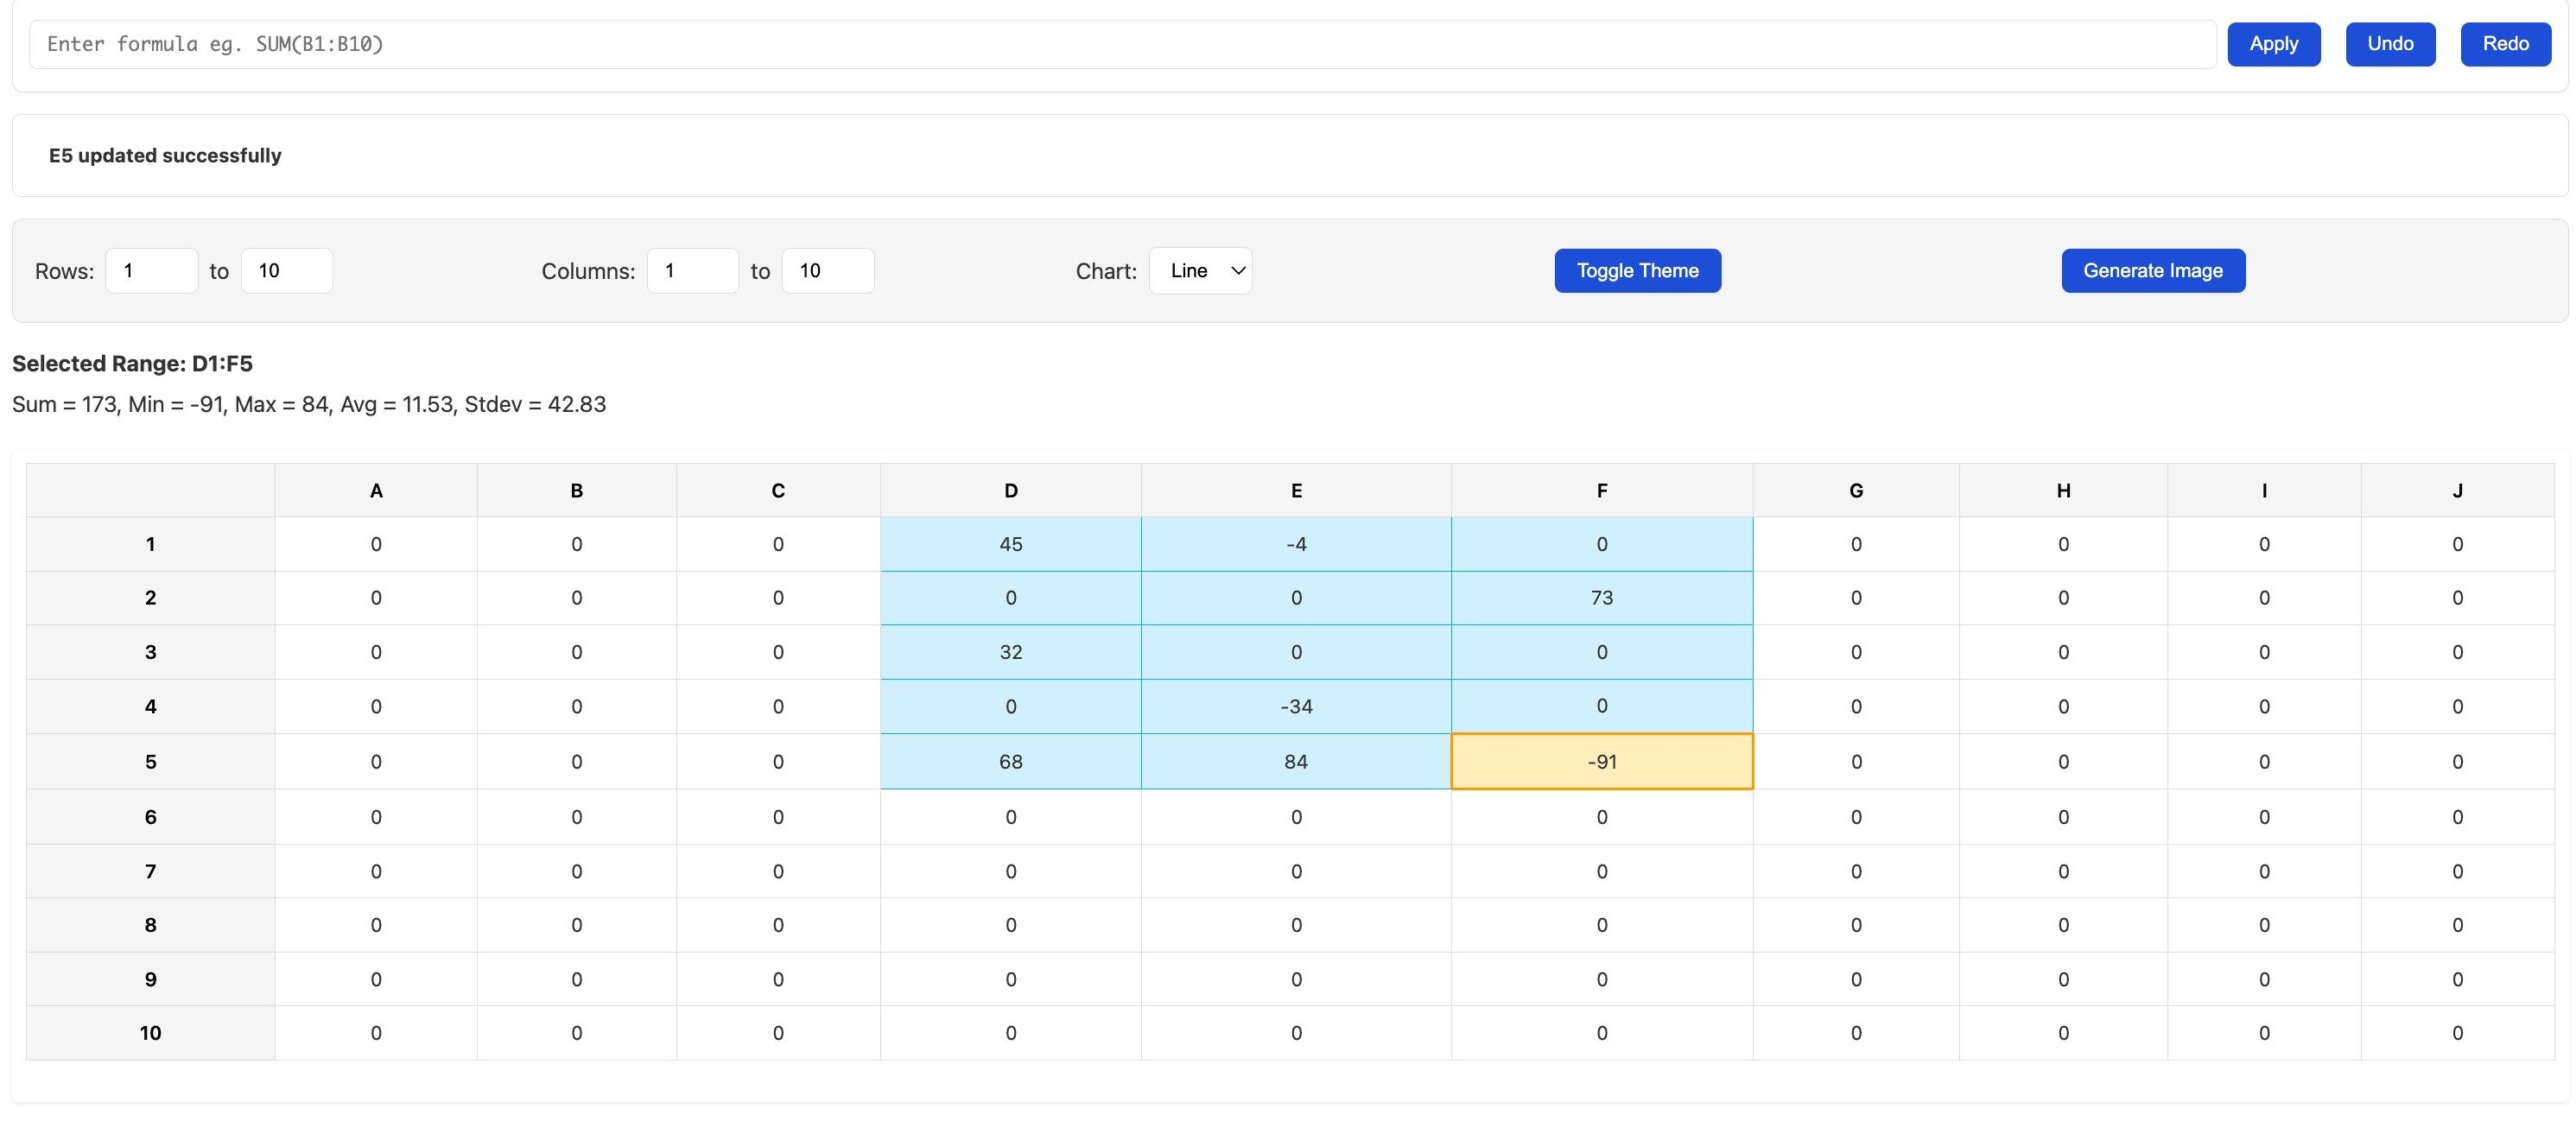
\includegraphics[width=9cm]{range.jpg}}}
    \caption{Range Data Analysis}
    \end{figure}
    \item Has a formula bar, which allows the user to change the value in a cell. This has an additional feature, where if a cell address appears in the formula for a cell value, then instead of having to type in the address, we can also choose to click on the cell in the table. This would print the cell address in the formula bar in position of the cursor.
    \item Allows undo and redo, by a depth of 1 command.
    \item Creates charts for columns. Clicking on a column header generates the chart for it above the table. This chart, by default, is a line chart, but can be switched to a bar chart from a drop down list.
    \begin{figure}[t]
    \centering
    {{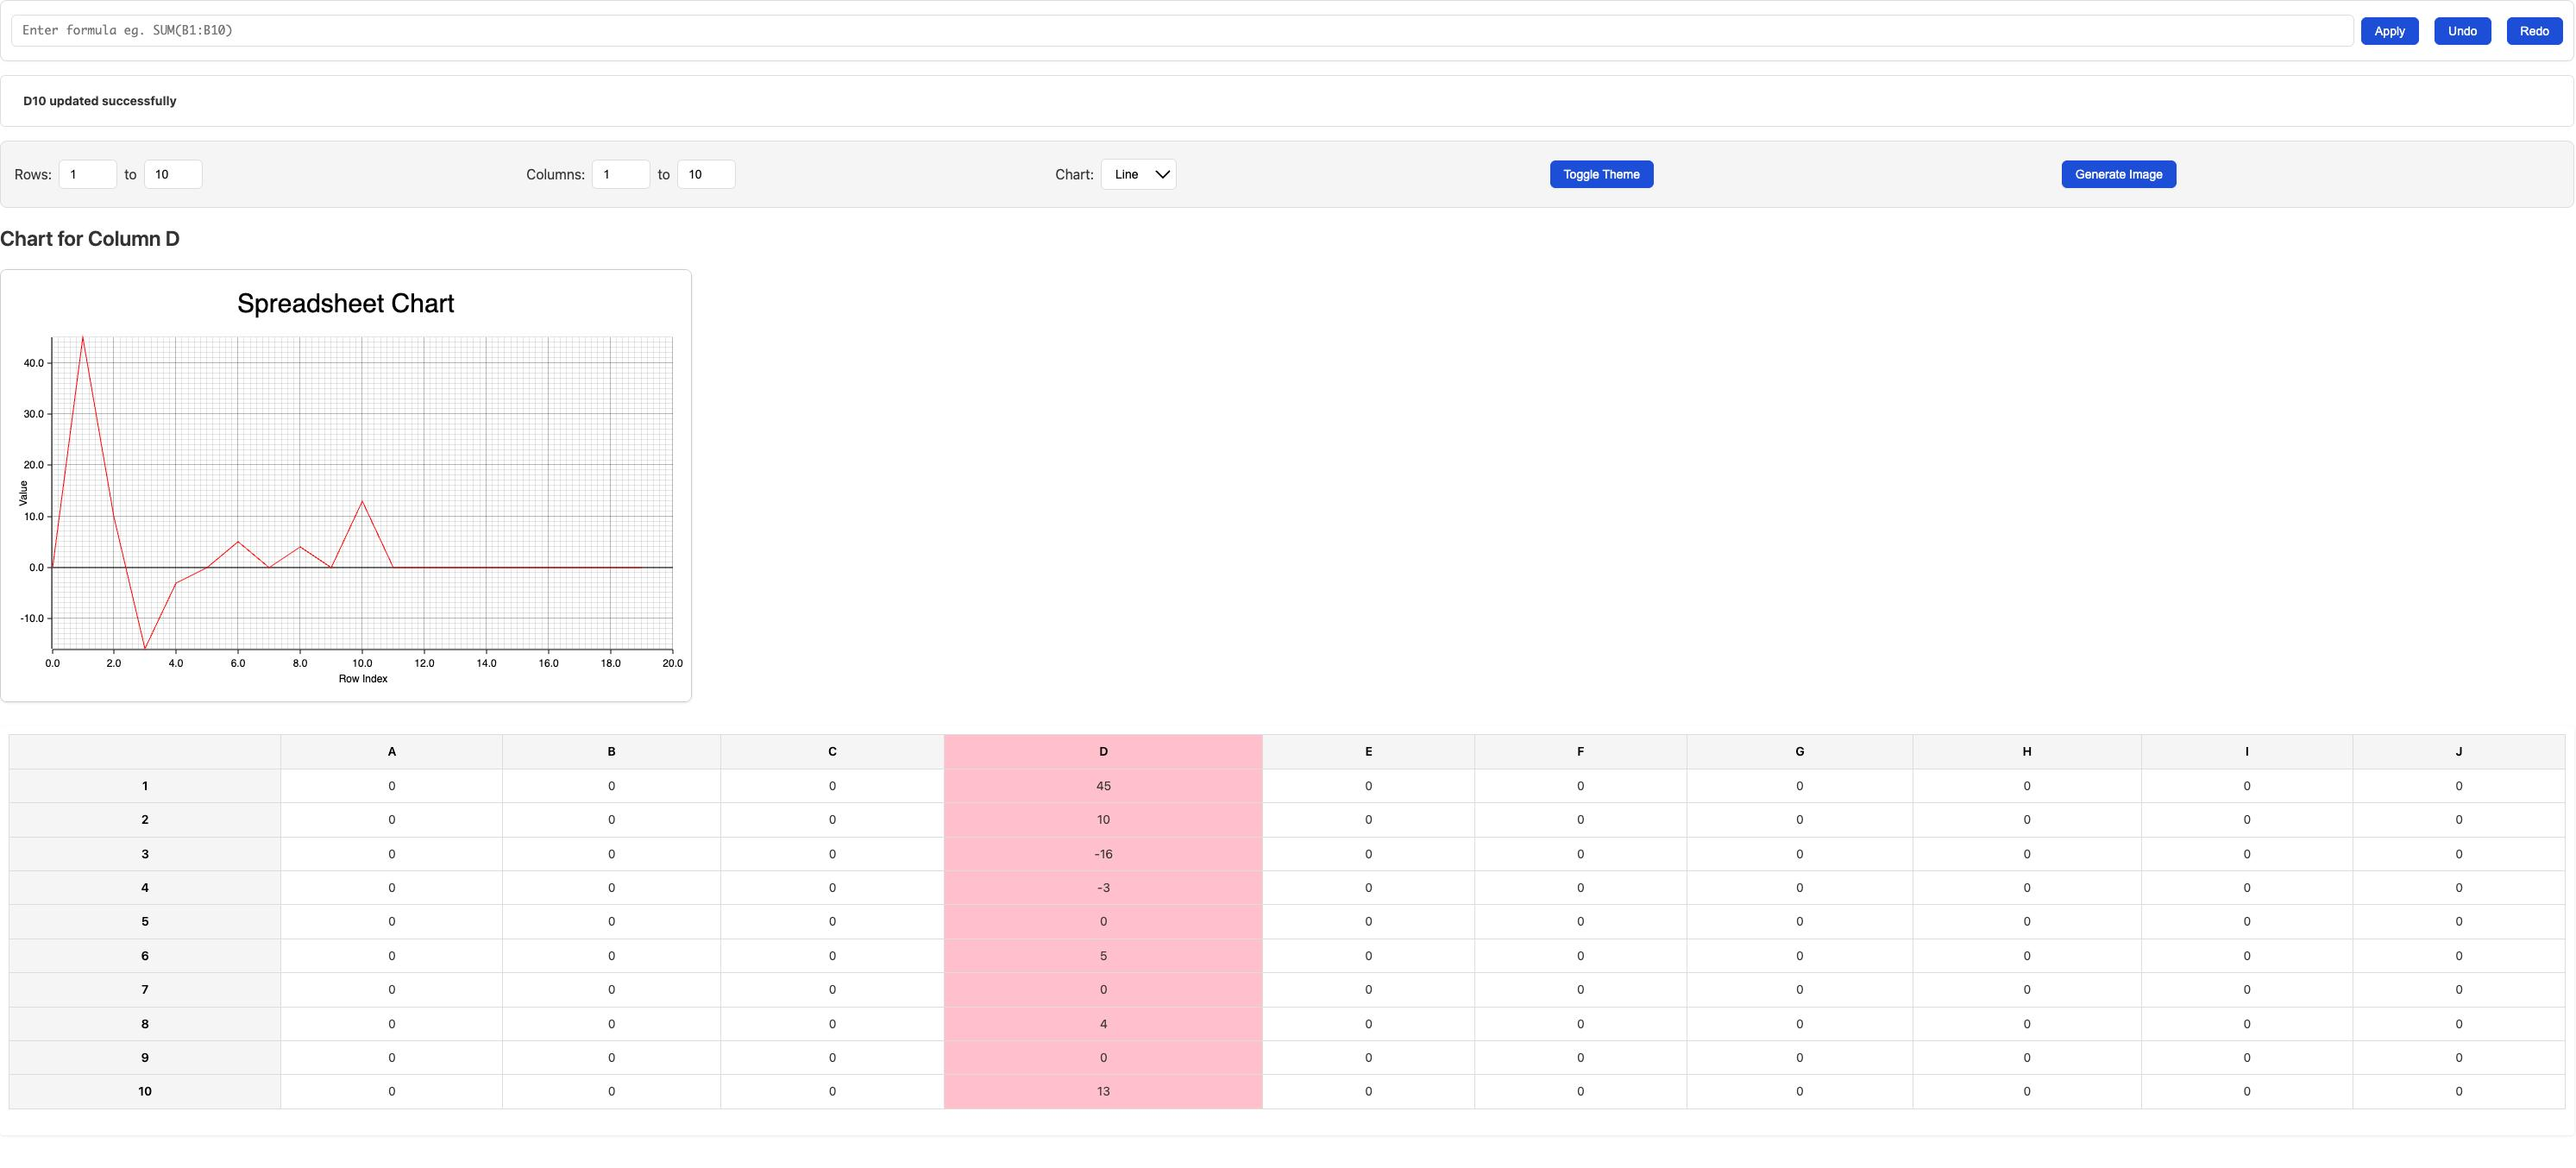
\includegraphics[width=9cm]{graph.jpg}}}
    \caption{Line Chart}
    \end{figure}
    \item Generates a heat map of the table. Maps the values inside a cell to an RGB value, using the following formula:
    $$((n>>16) \&\& (0xFF), (n>>8) \&\& (0xFF), n \&\& 0xFF)$$
    Any number which breaches the upper limit of numbers mappable to RGB values is mapped to the highest value, i.e., 0xFFFFFF (white). The maximum value is 16,777,215.
    \item Provides option for choosing between dark and light themes.
    \begin{figure}[t]
    \centering
    {{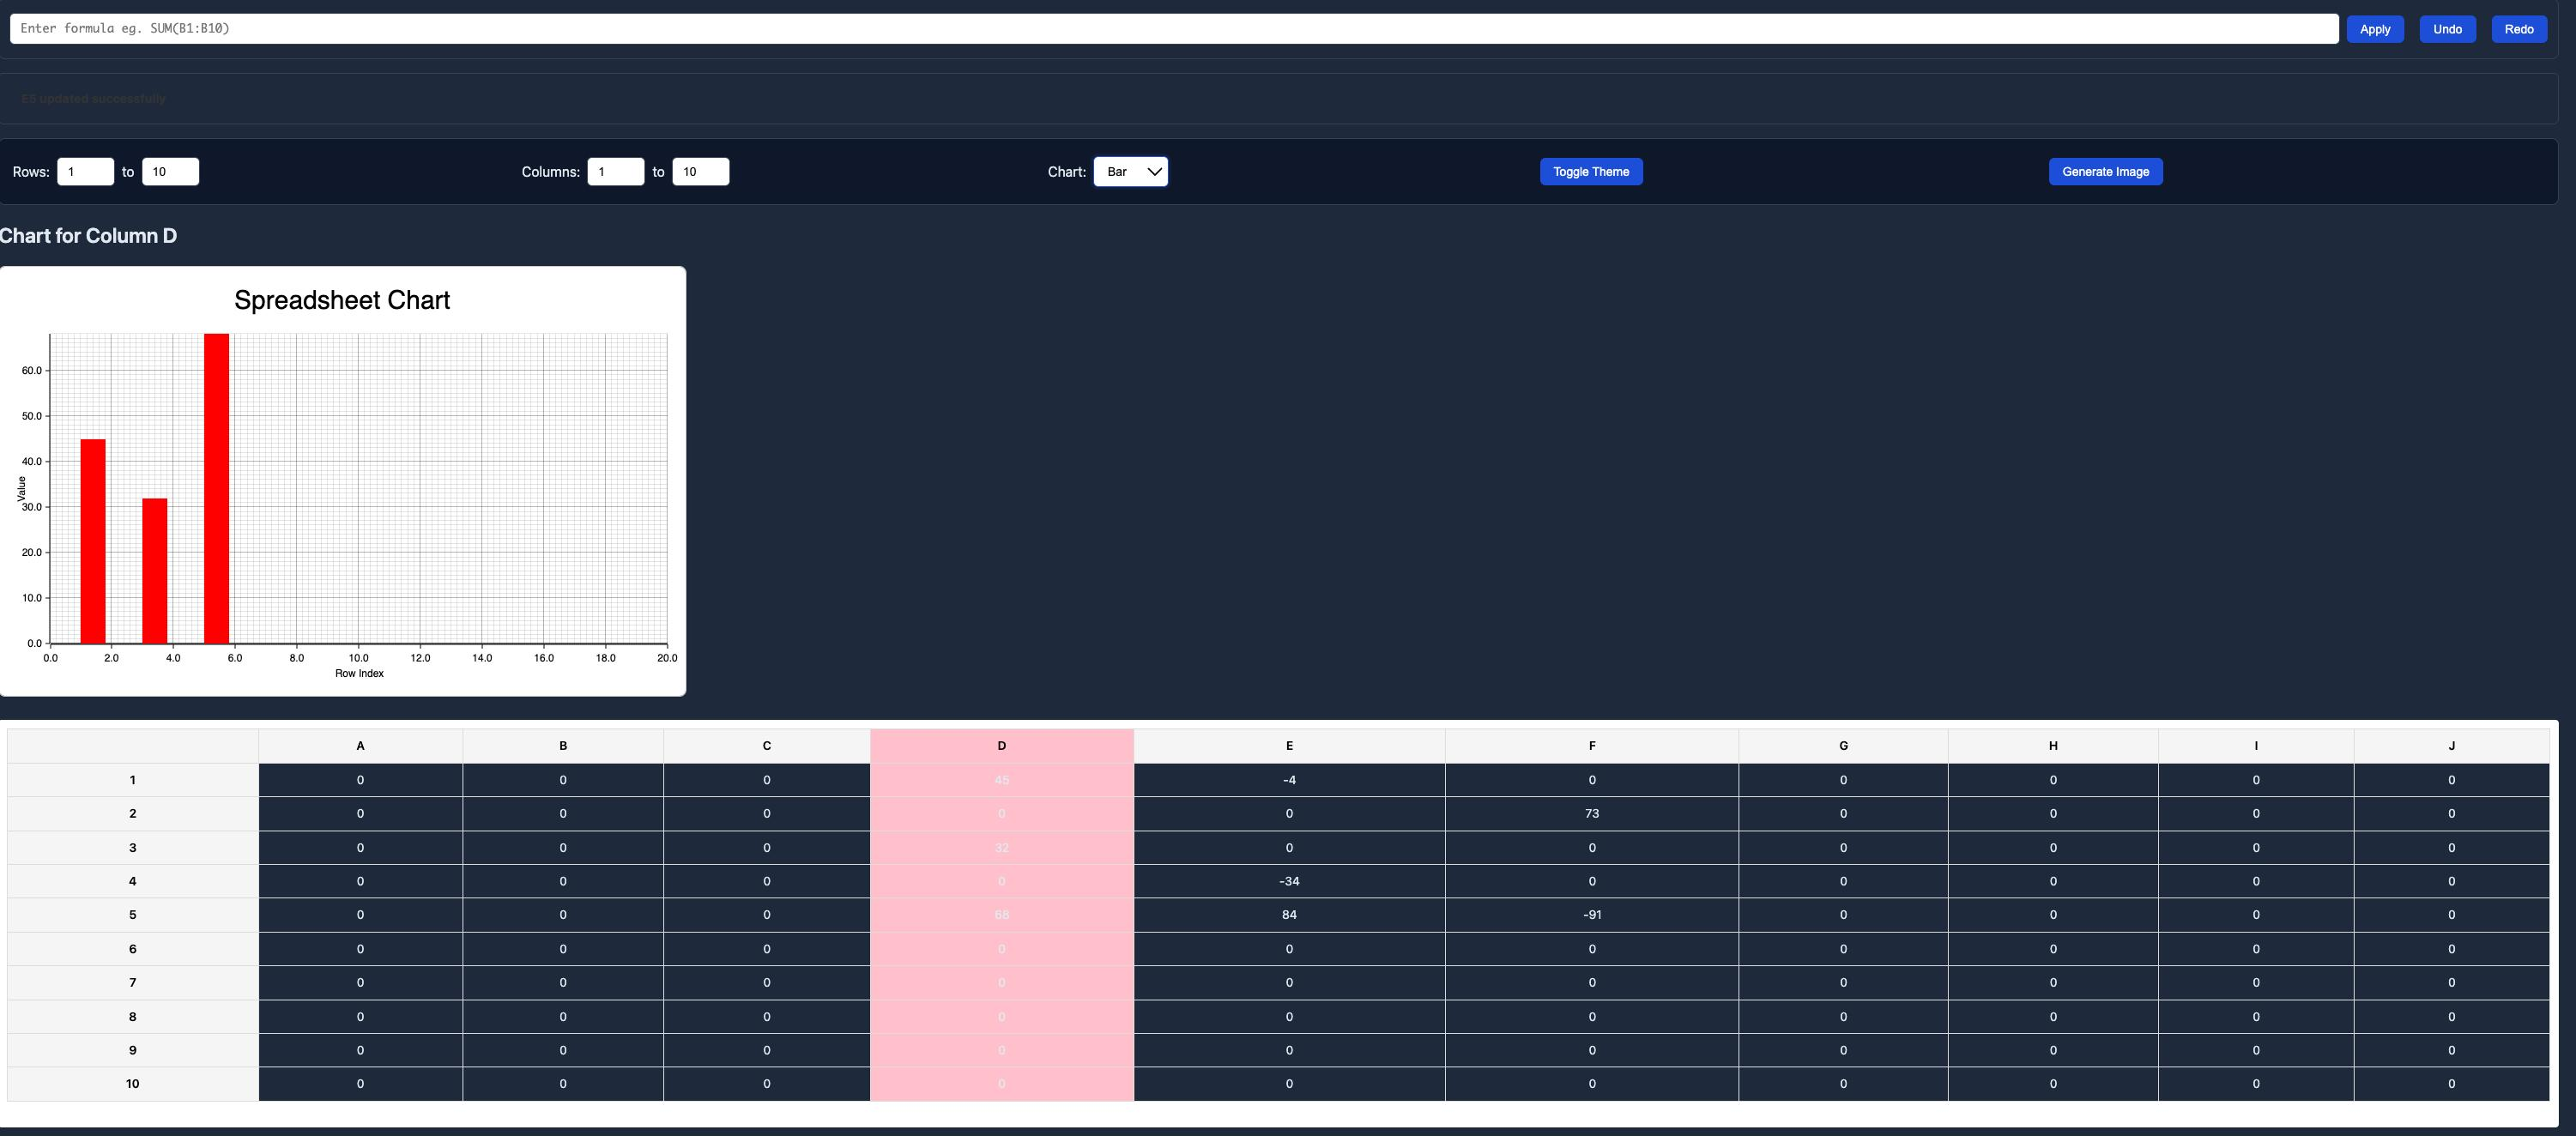
\includegraphics[width=9cm]{theme.jpg}}}
    \caption{Dark Theme}
    \end{figure}
\end{enumerate}

\section{Test Suite}

Our Rust project features a comprehensive and automated test suite, leveraging Rust's unit testing framework to ensure correctness, robustness, and maintainability of both terminal and web spreadsheet implementations. Tests are organized within each module using the \texttt{#[test]} macro, following Rust best practices.

\begin{enumerate}
    \item \textbf{Core Functionality:}
    \begin{itemize}
        \item \textbf{Arithmetic and Range Functions:} All spreadsheet functions (SUM, AVG, MIN, MAX, STDEV, etc.) are covered by unit tests. These tests verify correct results for single cells, rows, columns, rectangles, and edge cases such as empty or invalid ranges, as well as cells containing invalid values.
        \item \textbf{Cell Operations:} Unit tests validate all arithmetic operations (addition, subtraction, multiplication, division), including correct handling of division by zero and propagation of invalid states.
        \item \textbf{Node and Grid Methods:} The \texttt{Node} struct's methods (get/set value, position, validity, dependencies) are thoroughly tested for correct behavior and edge cases.
    \end{itemize}

    \item \textbf{Dependency Graph and Cycle Detection:}
    \begin{itemize}
        \item \textbf{Dependency Management:} Tests confirm that adding and breaking dependency edges between cells works as intended for both binary and range-based operations.
        \item \textbf{Cycle Detection:} Both direct and indirect cycles are tested. The suite ensures that attempts to create cycles (e.g., $A1 \rightarrow B1 \rightarrow C1 \rightarrow A1$) are detected and prevented, and that the spreadsheet remains consistent after such operations.
        \item \textbf{Topological Updates:} Tests verify correct propagation of updates through the dependency graph, including topological sorting and resetting of traversal flags.
    \end{itemize}

    \item \textbf{Parser and Command Validation:}
    \begin{itemize}
        \item \textbf{Valid Commands:} The parser is tested for correct interpretation of valid cell assignments, arithmetic expressions, range functions, and special commands (undo, redo, navigation, save, web, etc.).
        \item \textbf{Invalid Inputs:} Extensive tests ensure that out-of-bound cell references, malformed commands, and invalid function names are gracefully rejected with appropriate error handling.
    \end{itemize}

    \item \textbf{Frontend and Navigation:}
    \begin{itemize}
        \item \textbf{Grid Display and Navigation:} Tests cover navigation commands (w/a/s/d), scrolling, and grid rendering, including edge cases at grid boundaries and toggling output display.
        \item \textbf{Frontend Initialization:} Both terminal and web frontends are tested for correct initialization, command processing, and integration with their respective backends.
    \end{itemize}

    \item \textbf{Web Extension Specific:}
    \begin{itemize}
        \item \textbf{Backend Logic:} The web backend is tested for grid creation, value assignment, undo/redo functionality, serialization/deserialization, and error reporting (e.g., invalid ranges, circular dependencies).
        \item \textbf{Frontend Integration:} Web frontend tests ensure correct navigation, grid display, and command execution, including edge cases and error handling.
    \end{itemize}

    \item \textbf{Special Features:}
    \begin{itemize}
        \item \textbf{Undo/Redo:} Tests verify that undo and redo commands correctly revert and reapply changes, maintaining spreadsheet consistency.
        \item \textbf{Serialization:} The suite includes tests for saving and loading spreadsheet state to and from files, ensuring data integrity.
        \item \textbf{Output Control:} Commands for enabling/disabling output are tested for correct frontend behavior.
    \end{itemize}

    \item \textbf{Error Handling:}
    \begin{itemize}
        \item \textbf{Division by Zero, Invalid Ranges, and Malformed Commands:} All error cases are tested to ensure the program does not panic and provides informative feedback to the user.
    \end{itemize}
\end{enumerate}

\noindent
The test suite is automated and can be run using \texttt{cargo test}, providing rapid feedback during development. This ensures high reliability and allows safe refactoring and extension of the codebase.


\section{Challenges Faced}
\begin{enumerate}
    \item Deciding the basic framework of the extension took some time.
    \item The basic framework and function signatures are necessary to be decided right from the beginning in a team-based project.
    \item We had to learn how to implement web using Rust.
    \item Adding features for Plotting graphs, Selecting range and Serialization took time.
    \item We faced challenge in integrating our basic terminal code with our extension (terminal + web)
    \item 'trunk Serve' command is not working on Baadal. We are spending a lot of time figuring that out.
\end{enumerate}


\section{Links}
\begin{enumerate}
    \item \textbf{Github}: \texttt{https://github.com/lakshgoel5/SpreadsheetRust.git}
\end{enumerate}

\end{document}